% !TeX spellcheck = en_GB 

\documentclass[a4paper, 12pt, oneside]{book}

\usepackage[english]{babel}
\usepackage[utf8]{inputenc}
\usepackage[pagestyles]{titlesec}
\usepackage{titletoc}
\usepackage{enumitem}
\usepackage{fancyhdr}
\usepackage[a4paper, margin = 2.5cm, headheight=14pt]{geometry}
\usepackage[hidelinks, colorlinks = false]{hyperref}
\usepackage[bottom]{footmisc}
\usepackage{bookmark}
\usepackage{fontspec}
\usepackage{graphicx}
\usepackage[labelfont = bf]{caption}
\usepackage{etoolbox}
\usepackage{tabularx}
\usepackage{colortbl}
\usepackage{float}

\usepackage[table]{xcolor}

\title{
	
\includegraphics[width=0.75\textwidth]{assets/logo.png}
	\\
	{\huge Hubbl, a gym bookings manager}
}
\author{Miquel de Domingo i Giralt}

\setmainfont{SF Pro Display}[BoldFont = SF Pro Display Bold]
\setmonofont[Scale=0.9]{JetBrains Mono}

\newfontfamily\semibf{SF Pro Display Semibold}

% Variable with the page that keeps the footer style
\def\footerstyle{- \fontsize{10pt}{10pt}\selectfont\thepage\ -}
\pagestyle{fancy}
% Remove the horizontal bar from the header
\renewcommand{\headrulewidth}{0pt}
% Clear everythihg
\fancyhf{}
% Set header style
\rhead{\small\textit{\nouppercase{\rightmark}}}
% Set the footer page number
\fancyfoot[C]{\footerstyle}
% Update the footer in chapter and other plain views
\fancypagestyle{plain}{%
    \renewcommand{\headrulewidth}{0pt}%
    \fancyhf{}%
    \fancyfoot[C]{\footerstyle}%
}

\setlength\parindent{0pt}
\setcounter{secnumdepth}{5}
\setcounter{tocdepth}{5}

% Tables format
\definecolor{rowColor}{RGB}{242, 242, 242}
\renewcommand{\arraystretch}{1.5}

\titleformat{\chapter}[hang]{\normalfont\huge\bfseries}{\thechapter. }{4pt}{\Huge}
\titlespacing{\chapter}{0pt}{-32pt}{12pt}

\begin{document}
\chapter{Planning}
This chapter will cover the planning of the project. After having defined the requirements and the matrix of dependencies of such requirements, working packages will be defined, which will ensure an organized development using tasks.
\section{Working packages}
Each's table corresponds to one of the working packages. Since the \emph{Development} branch of the working packages tree the most extensive, its tables are explained after the \emph{Testing} branch, and so are the package numbers.
\begin{figure}[H]
	\centering
	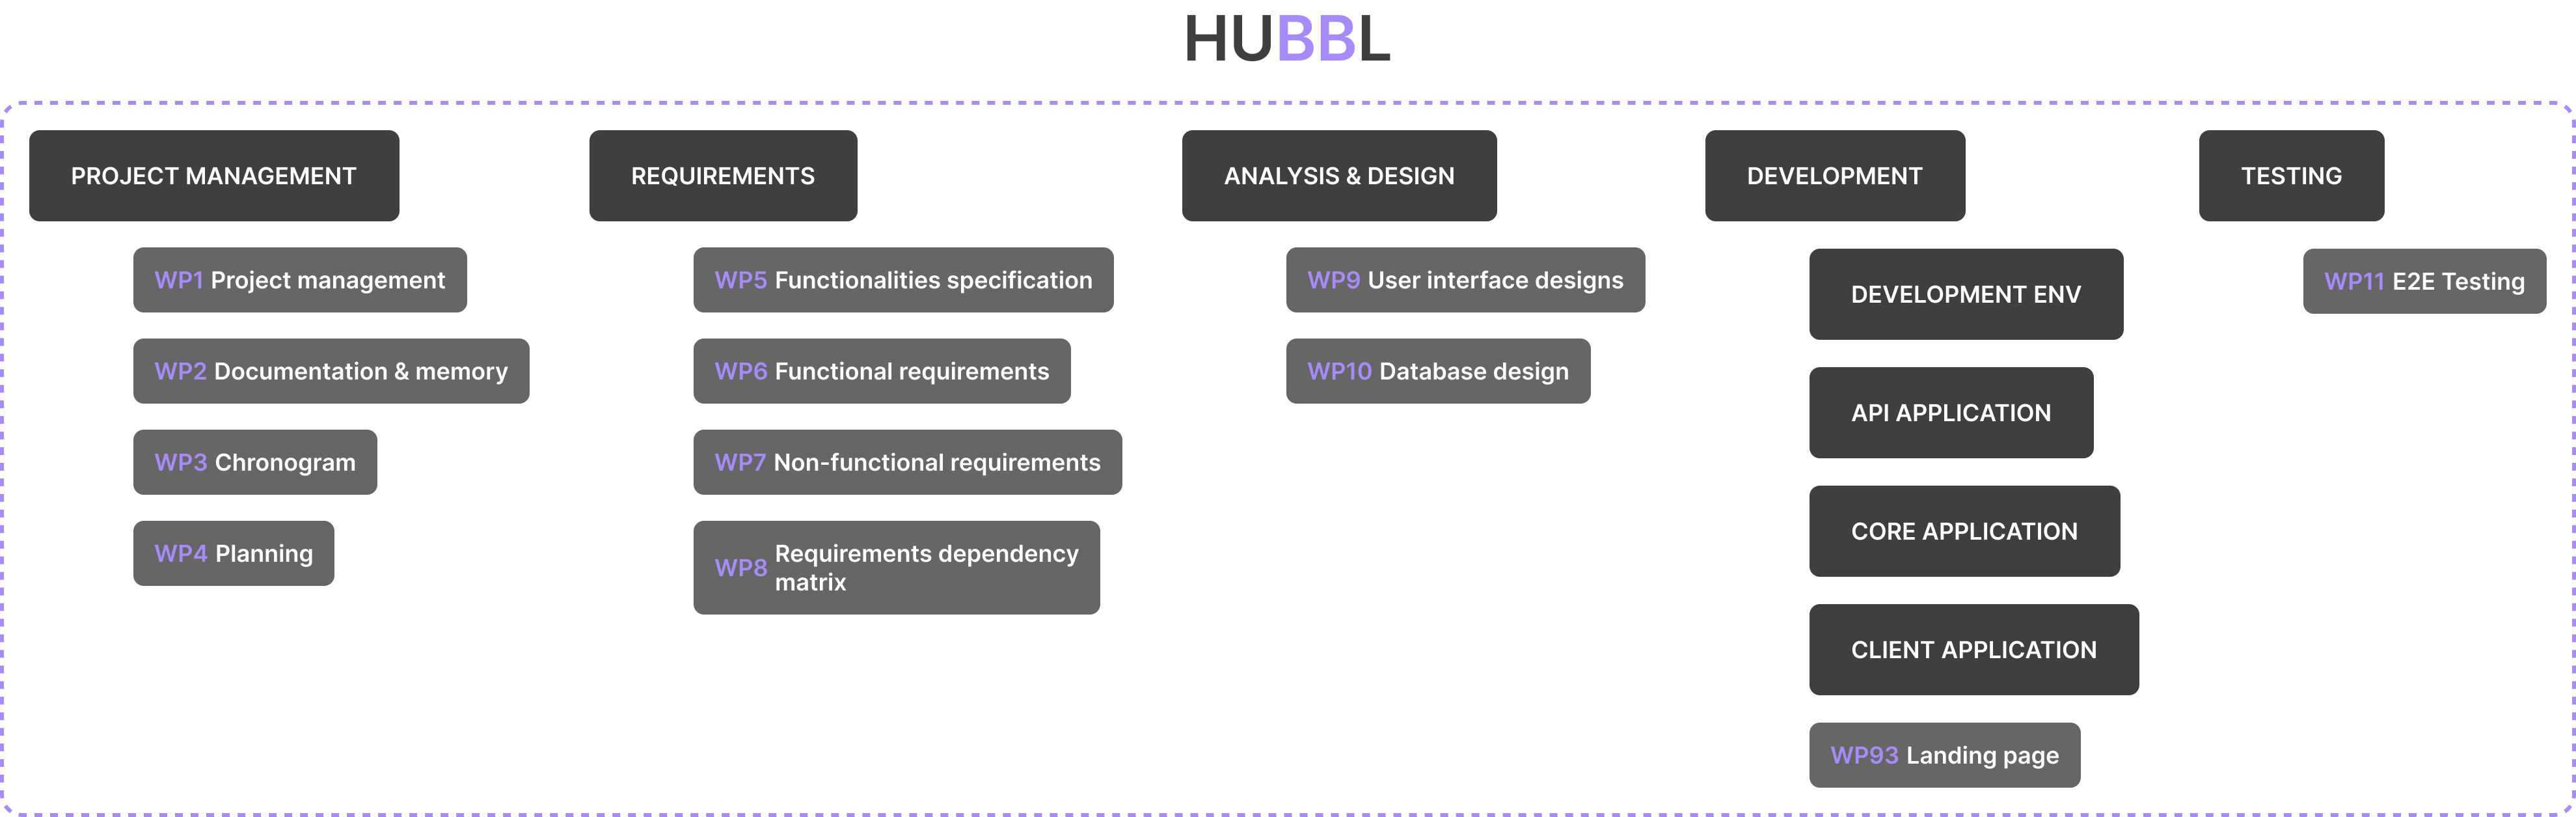
\includegraphics[width=\textwidth]{assets/working-packages/All.png}
	\caption{Structure of the working packages at the root level}
\end{figure}
The image above shows how the working packages have been organized. Each column represents a module, which are:
\begin{enumerate}[label = -]
	\item Project management.
	\item Requirements.
	\item Analysis and design.
	\item Development.
	\item Testing.
\end{enumerate}
Since the development branch is very extensive, each project has been extracted in smaller working packages.
\subsection{Project management}
The \emph{project management} branch contains all the working packages that are related any task that involves the specification of how the project will be managed in order to be successful.
\\[8pt]
\begin{tabularx}{\textwidth}{| l | X |}
	\hline
	\rowcolor{rowColor}
	{\semibf Package name}   & {\semibf WP1}: Project management             \\
	\hline
	{\semibf Description}    & Working package description.                  \\
	\hline
	\rowcolor{rowColor}
	{\semibf Estimated time} & 1d                                            \\
	\hline
	{\semibf Tasks}          & {\semibf T1}: Project document writing.
	\newline {\semibf T2}: Project document review.                          \\
	\hline
	\rowcolor{rowColor}
	{\semibf Results}        & Project document to be submitted to the jury. \\
	\hline
\end{tabularx}
\captionof{table}{Package one's table - Project management}
\vspace*{16pt}
\begin{tabularx}{\textwidth}{| l | X |}
	\hline
	\rowcolor{rowColor}
	{\semibf Package name}   & {\semibf WP2}: Documentation and memory            \\
	\hline
	{\semibf Description}    & Wording of some chapters of the memory.            \\
	\hline
	\rowcolor{rowColor}
	{\semibf Estimated time} & 4d                                                 \\
	\hline
	{\semibf Tasks}          & {\semibf T1}: Wording of the project introduction.
	\newline {\semibf T2}: Wording of the requirements.
	\newline {\semibf T3}: Wording of the analysis and design.
	\newline {\semibf T4}: Wording of the studies and decisions.
	\newline {\semibf T5}: Wording of the project development.                    \\
	\hline
	\rowcolor{rowColor}
	{\semibf Results}        & Project document to be submitted to the jury.      \\
	\hline
\end{tabularx}
\captionof{table}{Package two's table - Documentation and memory}
\vspace*{16pt}
\begin{tabularx}{\textwidth}{| l | X |}
	\hline
	\rowcolor{rowColor}
	{\semibf Package name}   & {\semibf WP3}: Chronogram                                  \\
	\hline
	{\semibf Description}    & Define the working chronogram for the project development. \\
	\hline
	\rowcolor{rowColor}
	{\semibf Estimated time} & 4h                                                         \\
	\hline
	{\semibf Tasks}          & {\semibf T1}: Temporal planning of the working packages.   \\
	\hline
	\rowcolor{rowColor}
	{\semibf Results}        & Gantt's project diagram.                                   \\
	\hline
\end{tabularx}
\captionof{table}{Package three's table - Chronogram}
\vspace*{16pt}
\begin{tabularx}{\textwidth}{| l | X |}
	\hline
	\rowcolor{rowColor}
	{\semibf Package name}   & {\semibf WP4}: Planning                         \\
	\hline
	{\semibf Description}    & Structure the working packages.                 \\
	\hline
	\rowcolor{rowColor}
	{\semibf Estimated time} & 4h                                              \\
	\hline
	{\semibf Tasks}          & {\semibf T1}: Planning of the working packages. \\
	\hline
	\rowcolor{rowColor}
	{\semibf Results}        & Chapter 6 of the memory document.               \\
	\hline
\end{tabularx}
\captionof{table}{Package four's table - Planning}
\vspace*{16pt}
\begin{tabularx}{\textwidth}{| l | X |}
	\hline
	\rowcolor{rowColor}
	{\semibf Package name}   & {\semibf WP5}: Functionalities specification        \\
	\hline
	{\semibf Description}    & Analysis of the functionalities of the application. \\
	\hline
	\rowcolor{rowColor}
	{\semibf Estimated time} & 8h                                                  \\
	\hline
	{\semibf Tasks}          & {\semibf T1}: Users identification.
	\newline {\semibf T2}: Define user needs (owner/worker and client).
	\newline {\semibf T3}: Define product functionalities                          \\
	\hline
	\rowcolor{rowColor}
	{\semibf Results}        & Sections 5.2 and 5.3 of the memory document.        \\
	\hline
\end{tabularx}
\captionof{table}{Package five's table - Functionalities specification}
\subsection{Requirements}
The \emph{requirements} branch contains all the tasks that are related with the analysis and definition of all the requirements and functionalities of each application.
\\[8pt]
\begin{tabularx}{\textwidth}{| l | X |}
	\hline
	\rowcolor{rowColor}
	{\semibf Package name}   & {\semibf WP6}: Functional requirements                                                 \\
	\hline
	{\semibf Description}    & Analysis and definition of the functional requirements of the application.             \\
	\hline
	\rowcolor{rowColor}
	{\semibf Estimated time} & 1d 4h\footnote{\emph{1d} is considered 1 day of work, which means a total of 8 hours.} \\
	\hline
	{\semibf Tasks}          & {\semibf T1}: Use case diagram.
	\newline {\semibf T2}: Functional requirements' specification for the \textit{core} application.
	\newline {\semibf T3}: Functional requirements' specification for the \textit{client} application.
	\newline {\semibf T4}: Functional requirements' specification for the \textit{landing} application.
	\newline {\semibf T5}: Functional requirements review and make changes if needed.                                 \\
	\hline
	\rowcolor{rowColor}
	{\semibf Results}        & Section 5.4 of the memory document.                                                    \\
	\hline
\end{tabularx}
\captionof{table}{Package six's table - Functional requirements}
\vspace*{16pt}
\begin{tabularx}{\textwidth}{| l | X |}
	\hline
	\rowcolor{rowColor}
	{\semibf Package name}   & {\semibf WP7}: Non-functional requirements                                     \\
	\hline
	{\semibf Description}    & Analysis and definition of the non-functional requirements of the application. \\
	\hline
	\rowcolor{rowColor}
	{\semibf Estimated time} & 4h                                                                             \\
	\hline
	{\semibf Tasks}          & {\semibf T1}: Initial non-functional requirements' specification.
	\newline {\semibf T2}: Non-functional requirements review and make changes if needed.                     \\
	\hline
	\rowcolor{rowColor}
	{\semibf Results}        & Section 5.5 of the memory document.                                            \\
	\hline
\end{tabularx}
\captionof{table}{Package seven's table - Non-functional requirements}
\vspace*{16pt}
\begin{tabularx}{\textwidth}{| l | X |}
	\hline
	\rowcolor{rowColor}
	{\semibf Package name}   & {\semibf WP8}: Requirements dependency matrix          \\
	\hline
	{\semibf Description}    & Definition of the requirements' dependency matrix.     \\
	\hline
	\rowcolor{rowColor}
	{\semibf Estimated time} & 4h                                                     \\
	\hline
	{\semibf Tasks}          & {\semibf T1}: Matrix dependency specification once the
	functional and non-functional requirements have been specified.                   \\
	\hline
	\rowcolor{rowColor}
	{\semibf Results}        & Section 5.6 of the memory document.                    \\
	\hline
\end{tabularx}
\captionof{table}{Package eight's table - Requirements dependency matrix}
\subsection{Analysis and design}
The \emph{analysis and design} branch contains all the working packages that are related with the design and analysis of the system interface and architecture.
\\[8pt]
\begin{tabularx}{\textwidth}{| l | X |}
	\hline
	\rowcolor{rowColor}
	{\semibf Package name}   & {\semibf WP9}: User interface designs                                 \\
	\hline
	{\semibf Description}    & Definition of the requirements' dependency matrix.                    \\
	\hline
	\rowcolor{rowColor}
	{\semibf Estimated time} & 12d                                                                   \\
	\hline
	{\semibf Tasks}          & {\semibf T1}: Design system specification.
	\newline {\semibf T2}: Prototype most of the user interfaces.
	\newline {\semibf T3}: Design review. Ensure it satisfies the requirements previously specified. \\
	\hline
	\rowcolor{rowColor}
	{\semibf Results}        & User interface prototypes which provide a vague view of the
	application's look and feel.                                                                     \\
	\hline
\end{tabularx}
\captionof{table}{Package nine's table - User interfaces designs}
\vspace*{16pt}
\begin{tabularx}{\textwidth}{| l | X |}
	\hline
	\rowcolor{rowColor}
	{\semibf Package name}   & {\semibf WP10}: Database design                                       \\
	\hline
	{\semibf Description}    & Definition of the application's database.                             \\
	\hline
	\rowcolor{rowColor}
	{\semibf Estimated time} & 4h                                                                    \\
	\hline
	{\semibf Tasks}          & {\semibf T1}: Design of the applications' database structure.
	\newline {\semibf T2}: Schema and structure review.
	\newline {\semibf T3}: Analysis of the database structure using PostgreSQL.                      \\
	\hline
	\rowcolor{rowColor}
	{\semibf Results}        & Database structure in which the application's data will be persisted. \\
	\hline
\end{tabularx}
\captionof{table}{Package ten - Database design}
\subsection{Testing}
The \emph{testing} branch contains the working package that is related with the testing of the application.
\\[8pt]
\begin{tabularx}{\textwidth}{| l | X |}
	\hline
	\rowcolor{rowColor}
	{\semibf Package name}   & {\semibf WP11}: E2e testing                                              \\
	\hline
	{\semibf Description}    & End-to-end testing implementation for the applications.                  \\
	\hline
	\rowcolor{rowColor}
	{\semibf Estimated time} & 4h                                                                       \\
	\hline
	{\semibf Tasks}          & {\semibf T1}: \emph{API} aplication e2e testing.
	\newline {\semibf T2}: \emph{Core} application e2e testing.
	\newline {\semibf T3}: \emph{Client} application e2e testing.
	\newline {\semibf T4}: \emph{Landing} application e2e testing.                                      \\
	\hline
	\rowcolor{rowColor}
	{\semibf Results}        & End-to-end tests which ensure the correct behaviour of each application,
	and that any futher new features and updates do not break the application.                          \\
	\hline
\end{tabularx}
\captionof{table}{Package eleven's table - E2e testing}
\subsection{Development}
The \emph{development} branch is probably the most extensive, as it is the most important part of the project. The branch consists of 73 working packages in total. Nevertheless, most of the packages follow the same structure. For instance, as it is seen in the \nameref{working-packages-api}, each web service package follows the same structure: a working package to create an entity, another one to update it, a third one to delete it, and a final one to fetch the entity. The structure is the same for each web service, which easily increases the number of working packages.
\\[8pt]
Following such structure has been extremely useful to simplify how are tasks managed and temporized. In order to organise the tasks, an \emph{AGILE} approach has been used, even though the project has been done all by myself. Each subgroup of the \emph{development} branch has been considered as an \emph{epic} and each working package as a \emph{story}, which has as many tasks as required. This approach has been used for each project and has made the development of the project easier to manage.
\\[8pt]
% TODO: Add Jira biblyography
In order to simplify the process of \emph{epic}, \emph{story} and \emph{task} creation, the Jira software from Atlassian has been used. It has been extremely useful as it can be integrated with many tools, one being GitHub, where the code is hosted. The GitHub integration provides a lot of utilities, yet one of the most important is the fact that it tracks your branches, commits and pull requests. Using the three elements, I have been able to automate the process of starting and completing tasks, alongside of the Jira automation. The following diagram, describes the workflow of the tasks inside Jira:
\\
\begin{figure}[H]
	\centering
	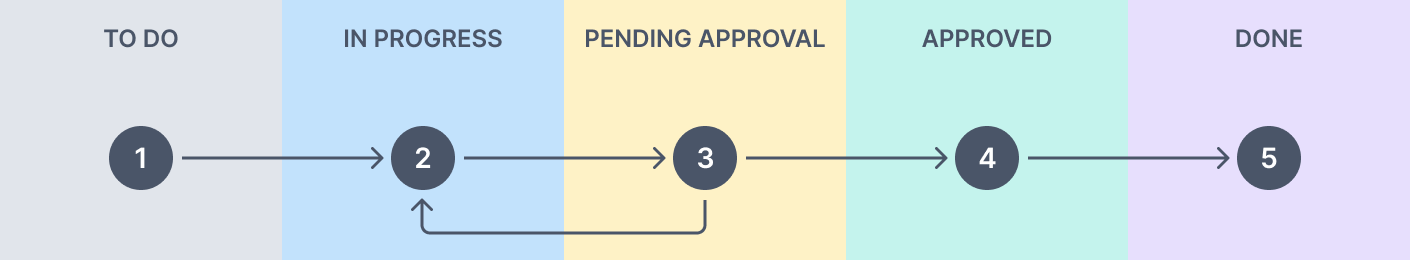
\includegraphics[width=\textwidth]{assets/working-packages/JiraWorkflow.png}
	\caption{5 steps of the Jira workflow}
\end{figure}
All the tasks would have to go from step 1 to step 5 in order to be considered as finished. Each step and the automation is as follows:
\begin{enumerate}
	\item All the tasks that have been selected for the sprint start at the first step, at the \emph{to-do} column.
	\item For each task, a new git branch has to be created with the name of the Jira task tag, for instance \texttt{HBL-185}\footnote{The \texttt{HBL} prefix is assigned when a new Jira project is created.}.
	      \\
	      When the branch is created and pushed to GitHub, Jira will move the task automatically to the \emph{in progress} column.
	      % TODO: Add Jira smart commits bibliography [21/03/2022]
	\item While in progress, each commit made is tracked in Jira. Additionally, Jira also supports \emph{smart commits} which are words prefixed with a hash (\#). With the smart commits, task properties can be changed. In this case, only the \texttt{\#time} has been used which increments the amount of time spent in each task. Tracking time has been useful to know more precisely how much time has been spent overall.
	\item Once the task is finished, a new pull request is made which triggers the continuous integration workflows set up at the GitHub repository. These workflows can also be watched by Jira and automate operations in function of the workflow result. If the task does not pass one of the workflows, the task is moved back to the \emph{in progress} tab. Alternatively, if the checks pass, it is moved to the \emph{approved} column.
	\item Finally, in order to be considered \emph{done}, the pull request of the task in question has to be merged. The merge will trigger another automated process which moves the task from \emph{approved} to \emph{done}.
\end{enumerate}
In order to stick to the process as much as possible, tasks moved to \emph{done}, should not be moved back. Instead, a new \emph{bug} type task was created which would start the process again.
\subsubsection{Development env}
The first group that is in the \emph{development} branch is the \emph{development env} (or \emph{development environment}). This part is as important as any other application, since it will define the structure of the project. Furthermore, the continuous integration has to be set up. Using the Nx build system, such feature becomes extremely simple and scalable. One of the options it offers is to run a command to as many projects as wanted. Not only so, that you can run the commands to the affected projects. Such feature reduces even more the CI execution time.
\begin{figure}[H]
	\centering
	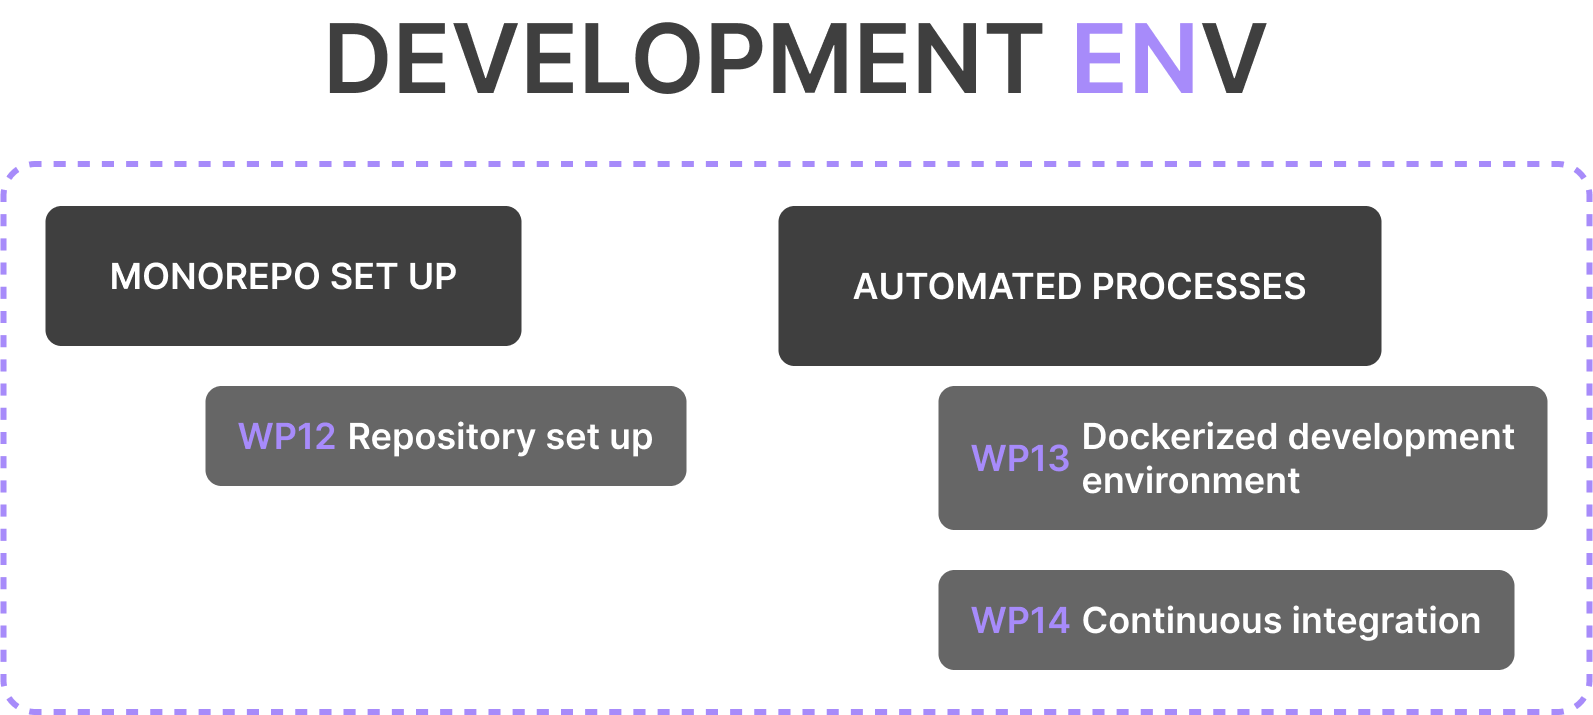
\includegraphics[width=\textwidth]{assets/working-packages/DevEnv.png}
	\caption{Api application working packages diagram}
\end{figure}
The \emph{development environment} group is composed of the following working packages:
\\[8pt]
\begin{tabularx}{\textwidth}{| l | X |}
	\hline
	\rowcolor{rowColor}
	{\semibf Package name}   & {\semibf WP12}: Repository set up                                 \\
	\hline
	{\semibf Description}    & Prepare the Nx monorepo.                                          \\
	\hline
	\rowcolor{rowColor}
	{\semibf Estimated time} & 2h                                                                \\
	\hline
	{\semibf Tasks}          & {\semibf T1}: Generate an \texttt{nx-workspace} ready to develop. \\
	\hline
	\rowcolor{rowColor}
	{\semibf Results}        & Initial structure of the monorepo.                                \\
	\hline
\end{tabularx}
\captionof{table}{Package twelve's table - Repository set up}
\vspace*{16pt}
\begin{tabularx}{\textwidth}{| l | X |}
	\hline
	\rowcolor{rowColor}
	{\semibf Package name}   & {\semibf WP13}: Dockerized development environment.                \\
	\hline
	{\semibf Description}    & Dockerize the database, the test database and the API application. \\
	\hline
	\rowcolor{rowColor}
	{\semibf Estimated time} & 2h                                                                 \\
	\hline
	{\semibf Tasks}          & {\semibf T1}: Dockerize the main database and the test database.
	\newline {\semibf T2}: Dockerize the API application using a NodeJS image.                    \\
	\hline
	\rowcolor{rowColor}
	{\semibf Results}        & The dockerization of the databases and the REST API.               \\
	\hline
\end{tabularx}
\captionof{table}{Package thirteen's table - Dockerized development environment}
\vspace*{16pt}
\begin{tabularx}{\textwidth}{| l | X |}
	\hline
	\rowcolor{rowColor}
	{\semibf Package name}   & {\semibf WP14}: Continuous integration.                 \\
	\hline
	{\semibf Description}    & Set up Github Actions for CI.                           \\
	\hline
	\rowcolor{rowColor}
	{\semibf Estimated time} & 1d                                                      \\
	\hline
	{\semibf Tasks}          & {\semibf T1}: Set up CI for the \emph{API} application.
	\newline {\semibf T2}: Set up CI for the \emph{core} application.
	\newline {\semibf T3}: Set up CI for the \emph{client} application.
	\newline {\semibf T4}: Set up CI for the \emph{landing} application.
	\newline {\semibf T5}: Set up CI for the monrepo libraries.                        \\
	\hline
	\rowcolor{rowColor}
	{\semibf Results}        & An automated process for testing the code developed.    \\
	\hline
\end{tabularx}
\captionof{table}{Package fourteen's table - Continuous integration}
\subsubsection{Api application}
\label{working-packages-api}
The working package groups of the \emph{api} application have been designed so that each web service of the application is divided in multiple working packages with tasks that are very specific and simple.
\begin{figure}[H]
	\centering
	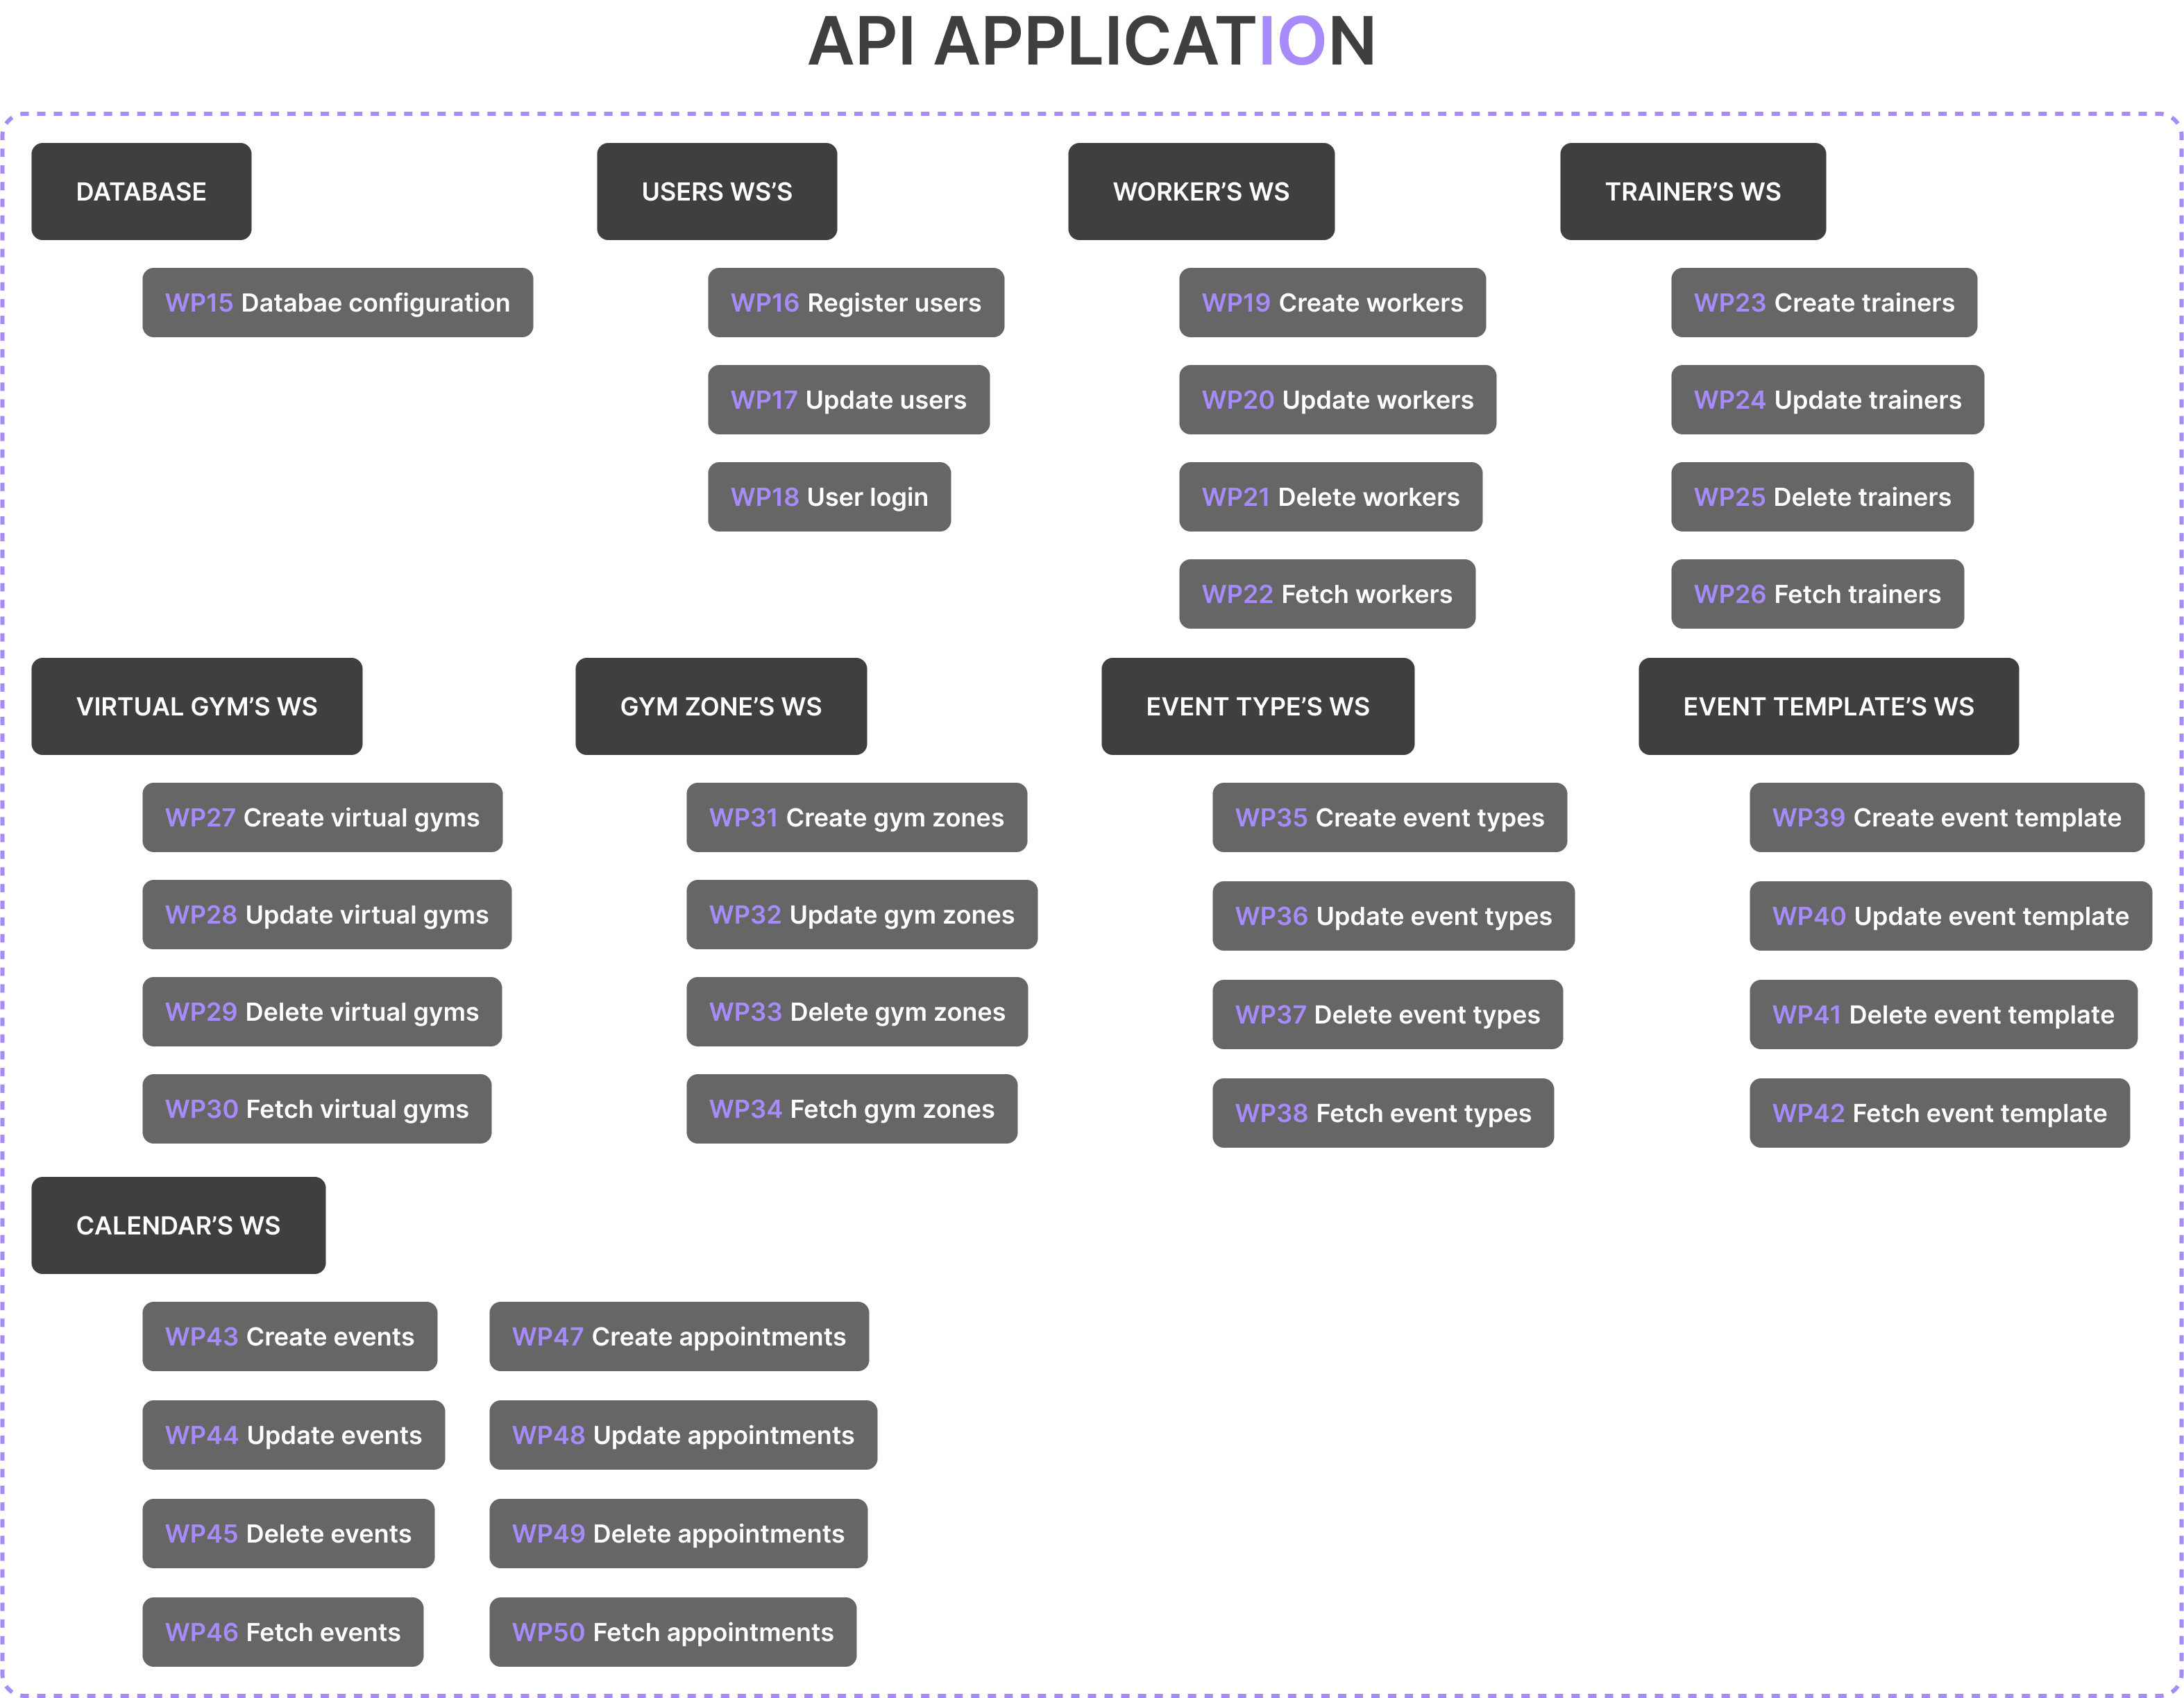
\includegraphics[width=\textwidth]{assets/working-packages/Api.png}
	\caption{Api application working packages diagram}
\end{figure}
The \emph{api} group is composed of the following working packages:
\\[8pt]
\begin{tabularx}{\textwidth}{| l | X |}
	\hline
	\rowcolor{rowColor}
	{\semibf Package name}   & {\semibf WP15}: Database configuration.                       \\
	\hline
	{\semibf Description}    & Configure the application so that is connected the database.  \\
	\hline
	\rowcolor{rowColor}
	{\semibf Estimated time} & 1h                                                            \\
	\hline
	{\semibf Tasks}          & {\semibf T1}: Configure the API with the dockerized database. \\
	\hline
	\rowcolor{rowColor}
	{\semibf Results}        & Connection of the api with the database.                      \\
	\hline
\end{tabularx}
\captionof{table}{Package fifteen's table - Database configuration}
\vspace*{16pt}
\begin{tabularx}{\textwidth}{| l | X |}
	\hline
	\rowcolor{rowColor}
	{\semibf Package name}   & {\semibf WP16}: Register users              \\
	\hline
	{\semibf Description}    & Allow the users to register.                \\
	\hline
	\rowcolor{rowColor}
	{\semibf Estimated time} & 1d                                          \\
	\hline
	{\semibf Tasks}          & {\semibf T1}: Create the services required.
	\newline {\semibf T2}: Create the controllers required.
	\newline {\semibf T3}: Create the owner register endpoint.
	\newline {\semibf T4}: Create the client register endpoint.            \\
	\hline
	\rowcolor{rowColor}
	{\semibf Results}        & Creation of a user.                         \\
	\hline
\end{tabularx}
\captionof{table}{Package sixteen's table - Register users}
\vspace*{16pt}
\begin{tabularx}{\textwidth}{| l | X |}
	\hline
	\rowcolor{rowColor}
	{\semibf Package name}   & {\semibf WP17}: Update users                 \\
	\hline
	{\semibf Description}    & Allow the users to update their information. \\
	\hline
	\rowcolor{rowColor}
	{\semibf Estimated time} & 4h                                           \\
	\hline
	{\semibf Tasks}          & {\semibf T1}: Create the services required.
	\newline {\semibf T2}: Create the controllers required.
	\newline {\semibf T3}: Create the user update endpoint.                 \\
	\hline
	\rowcolor{rowColor}
	{\semibf Results}        & Updation of user's information               \\
	\hline
\end{tabularx}
\captionof{table}{Package seventeen's table - Update users}
\vspace*{16pt}
\begin{tabularx}{\textwidth}{| l | X |}
	\hline
	\rowcolor{rowColor}
	{\semibf Package name}   & {\semibf WP18}: User login                         \\
	\hline
	{\semibf Description}    & Allow the users to log in to the application.      \\
	\hline
	\rowcolor{rowColor}
	{\semibf Estimated time} & 8h                                                 \\
	\hline
	{\semibf Tasks}          & {\semibf T1}: Create the services required.
	\newline {\semibf T2}: Create the controllers required.
	\newline {\semibf T3}: Create the session cookie validation endpoint.
	\newline {\semibf T4}: Create the login endpoint.                             \\
	\hline
	\rowcolor{rowColor}
	{\semibf Results}        & Endpoints to login and validate old user sessions. \\
	\hline
\end{tabularx}
\captionof{table}{Package eighteen's table - User login}
\vspace*{16pt}
\begin{tabularx}{\textwidth}{| l | X |}
	\hline
	\rowcolor{rowColor}
	{\semibf Package name}   & {\semibf WP19}: Create workers              \\
	\hline
	{\semibf Description}    & Allow the creation of workers.              \\
	\hline
	\rowcolor{rowColor}
	{\semibf Estimated time} & 6h                                          \\
	\hline
	{\semibf Tasks}          & {\semibf T1}: Create the services required.
	\newline {\semibf T2}: Create the controllers required.
	\newline {\semibf T3}: Create the workers create endpoint.             \\
	\hline
	\rowcolor{rowColor}
	{\semibf Results}        & Creation of workers.                        \\
	\hline
\end{tabularx}
\captionof{table}{Package nineteen's table - Create workers}
\vspace*{16pt}
\begin{tabularx}{\textwidth}{| l | X |}
	\hline
	\rowcolor{rowColor}
	{\semibf Package name}   & {\semibf WP20}: Update workers              \\
	\hline
	{\semibf Description}    & Allow the update of workers.                \\
	\hline
	\rowcolor{rowColor}
	{\semibf Estimated time} & 4h                                          \\
	\hline
	{\semibf Tasks}          & {\semibf T1}: Create the services required.
	\newline {\semibf T2}: Create the controllers required.
	\newline {\semibf T3}: Create the update workers endpoint.             \\
	\hline
	\rowcolor{rowColor}
	{\semibf Results}        & Updation of workers.                        \\
	\hline
\end{tabularx}
\captionof{table}{Package twenty's table - Update workers}
\begin{tabularx}{\textwidth}{| l | X |}
	\hline
	\rowcolor{rowColor}
	{\semibf Package name}   & {\semibf WP21}: Delete workers              \\
	\hline
	{\semibf Description}    & Allow the deletion of workers.              \\
	\hline
	\rowcolor{rowColor}
	{\semibf Estimated time} & 4h                                          \\
	\hline
	{\semibf Tasks}          & {\semibf T1}: Create the services required.
	\newline {\semibf T2}: Create the controllers required.
	\newline {\semibf T3}: Create the delete workers endpoint.             \\
	\hline
	\rowcolor{rowColor}
	{\semibf Results}        & Deletion of workers.                        \\
	\hline
\end{tabularx}
\captionof{table}{Package twenty-one's table - Delete workers}
\vspace*{16pt}
\begin{tabularx}{\textwidth}{| l | X |}
	\hline
	\rowcolor{rowColor}
	{\semibf Package name}   & {\semibf WP22}: Fetch workers               \\
	\hline
	{\semibf Description}    & Allow the fetch of workers.                 \\
	\hline
	\rowcolor{rowColor}
	{\semibf Estimated time} & 4h                                          \\
	\hline
	{\semibf Tasks}          & {\semibf T1}: Create the services required.
	\newline {\semibf T2}: Create the controllers required.
	\newline {\semibf T3}: Create the fetch workers endpoint.              \\
	\hline
	\rowcolor{rowColor}
	{\semibf Results}        & Fetching of workers.                        \\
	\hline
\end{tabularx}
\captionof{table}{Package twenty-two's table - Fetch workers}
\vspace*{16pt}
\begin{tabularx}{\textwidth}{| l | X |}
	\hline
	\rowcolor{rowColor}
	{\semibf Package name}   & {\semibf WP23}: Create trainers             \\
	\hline
	{\semibf Description}    & Allow the creation of trainers.             \\
	\hline
	\rowcolor{rowColor}
	{\semibf Estimated time} & 8h                                          \\
	\hline
	{\semibf Tasks}          & {\semibf T1}: Create the services required.
	\newline {\semibf T2}: Create the controllers required.
	\newline {\semibf T3}: Create the create trainers endpoint.            \\
	\hline
	\rowcolor{rowColor}
	{\semibf Results}        & Creation of trainers.                       \\
	\hline
\end{tabularx}
\captionof{table}{Package twenty-three's table - Create trainers}
\vspace*{16pt}
\begin{tabularx}{\textwidth}{| l | X |}
	\hline
	\rowcolor{rowColor}
	{\semibf Package name}   & {\semibf WP24}: Update trainers             \\
	\hline
	{\semibf Description}    & Allow the update of trainers.               \\
	\hline
	\rowcolor{rowColor}
	{\semibf Estimated time} & 4h                                          \\
	\hline
	{\semibf Tasks}          & {\semibf T1}: Create the services required.
	\newline {\semibf T2}: Create the controllers required.
	\newline {\semibf T3}: Create the update trainers endpoint.            \\
	\hline
	\rowcolor{rowColor}
	{\semibf Results}        & Updation of trainers.                       \\
	\hline
\end{tabularx}
\captionof{table}{Package twenty-four's table - Update trainers}
\vspace*{16pt}
\begin{tabularx}{\textwidth}{| l | X |}
	\hline
	\rowcolor{rowColor}
	{\semibf Package name}   & {\semibf WP25}: Delete trainers             \\
	\hline
	{\semibf Description}    & Allow the deletion of trainers.             \\
	\hline
	\rowcolor{rowColor}
	{\semibf Estimated time} & 4h                                          \\
	\hline
	{\semibf Tasks}          & {\semibf T1}: Create the services required.
	\newline {\semibf T2}: Create the controllers required.
	\newline {\semibf T3}: Create the delete trainers endpoint.            \\
	\hline
	\rowcolor{rowColor}
	{\semibf Results}        & Deletion of trainers.                       \\
	\hline
\end{tabularx}
\captionof{table}{Package twenty-five's table - Delete trainers}
\vspace*{16pt}
\begin{tabularx}{\textwidth}{| l | X |}
	\hline
	\rowcolor{rowColor}
	{\semibf Package name}   & {\semibf WP26}: Fetch trainers              \\
	\hline
	{\semibf Description}    & Allow the fetch of trainers.                \\
	\hline
	\rowcolor{rowColor}
	{\semibf Estimated time} & 4h                                          \\
	\hline
	{\semibf Tasks}          & {\semibf T1}: Create the services required.
	\newline {\semibf T2}: Create the controllers required.
	\newline {\semibf T3}: Create the fetch trainers endpoint.             \\
	\hline
	\rowcolor{rowColor}
	{\semibf Results}        & Fetching of trainers.                       \\
	\hline
\end{tabularx}
\captionof{table}{Package twenty-six's table - Fetch trainers}
\vspace*{16pt}
\begin{tabularx}{\textwidth}{| l | X |}
	\hline
	\rowcolor{rowColor}
	{\semibf Package name}   & {\semibf WP27}: Create virtual gyms         \\
	\hline
	{\semibf Description}    & Allow the creation of virtual gyms.         \\
	\hline
	\rowcolor{rowColor}
	{\semibf Estimated time} & 8h                                          \\
	\hline
	{\semibf Tasks}          & {\semibf T1}: Create the services required.
	\newline {\semibf T2}: Create the controllers required.
	\newline {\semibf T3}: Create the virtual gym creation endpoint.       \\
	\hline
	\rowcolor{rowColor}
	{\semibf Results}        & Creation of virtual gyms.                   \\
	\hline
\end{tabularx}
\captionof{table}{Package twenty-seven's table - Create virtual gyms}
\vspace*{16pt}
\begin{tabularx}{\textwidth}{| l | X |}
	\hline
	\rowcolor{rowColor}
	{\semibf Package name}   & {\semibf WP28}: Update virtual gyms         \\
	\hline
	{\semibf Description}    & Allow the update of virtual gyms.           \\
	\hline
	\rowcolor{rowColor}
	{\semibf Estimated time} & 4h                                          \\
	\hline
	{\semibf Tasks}          & {\semibf T1}: Create the services required.
	\newline {\semibf T2}: Create the controllers required.
	\newline {\semibf T3}: Create the virtual gym update endpoint.         \\
	\hline
	\rowcolor{rowColor}
	{\semibf Results}        & Updation of virtual gyms.                   \\
	\hline
\end{tabularx}
\captionof{table}{Package twenty-eight's table - Update virtual gyms}
\vspace*{16pt}
\begin{tabularx}{\textwidth}{| l | X |}
	\hline
	\rowcolor{rowColor}
	{\semibf Package name}   & {\semibf WP29}: Delete virtual gyms         \\
	\hline
	{\semibf Description}    & Allow the deletion of virtual gyms.         \\
	\hline
	\rowcolor{rowColor}
	{\semibf Estimated time} & 4h                                          \\
	\hline
	{\semibf Tasks}          & {\semibf T1}: Create the services required.
	\newline {\semibf T2}: Create the controllers required.
	\newline {\semibf T3}: Create the virtual gym deletion endpoint.       \\
	\hline
	\rowcolor{rowColor}
	{\semibf Results}        & Deletion of virtual gyms.                   \\
	\hline
\end{tabularx}
\captionof{table}{Package twenty-nine's table - Delete virtual gyms}
\vspace*{16pt}
\begin{tabularx}{\textwidth}{| l | X |}
	\hline
	\rowcolor{rowColor}
	{\semibf Package name}   & {\semibf WP30}: Fetch virtual gyms          \\
	\hline
	{\semibf Description}    & Allow the fetch of virtual gyms.            \\
	\hline
	\rowcolor{rowColor}
	{\semibf Estimated time} & 4h                                          \\
	\hline
	{\semibf Tasks}          & {\semibf T1}: Create the services required.
	\newline {\semibf T2}: Create the controllers required.
	\newline {\semibf T3}: Create the virtual gym fetch endpoint.          \\
	\hline
	\rowcolor{rowColor}
	{\semibf Results}        & Fetching of virtual gyms.                   \\
	\hline
\end{tabularx}
\captionof{table}{Package thirty's table - Delete virtual gyms}
\vspace*{16pt}
\begin{tabularx}{\textwidth}{| l | X |}
	\hline
	\rowcolor{rowColor}
	{\semibf Package name}   & {\semibf WP31}: Create gym zones            \\
	\hline
	{\semibf Description}    & Allow the creation of gym zones.            \\
	\hline
	\rowcolor{rowColor}
	{\semibf Estimated time} & 8h                                          \\
	\hline
	{\semibf Tasks}          & {\semibf T1}: Create the services required.
	\newline {\semibf T2}: Create the controllers required.
	\newline {\semibf T3}: Create the gym zone create endpoint.            \\
	\hline
	\rowcolor{rowColor}
	{\semibf Results}        & Creation of gym zones.                      \\
	\hline
\end{tabularx}
\captionof{table}{Package thirty-one's table - Create gym zones}
\vspace*{16pt}
\begin{tabularx}{\textwidth}{| l | X |}
	\hline
	\rowcolor{rowColor}
	{\semibf Package name}   & {\semibf WP32}: Update gym zones            \\
	\hline
	{\semibf Description}    & Allow the update of gym zones.              \\
	\hline
	\rowcolor{rowColor}
	{\semibf Estimated time} & 4h                                          \\
	\hline
	{\semibf Tasks}          & {\semibf T1}: Create the services required.
	\newline {\semibf T2}: Create the controllers required.
	\newline {\semibf T3}: Create the gym zone update endpoint.            \\
	\hline
	\rowcolor{rowColor}
	{\semibf Results}        & Updation of gym zones.                      \\
	\hline
\end{tabularx}
\captionof{table}{Package thirty-two's table - Update gym zones}
\vspace*{16pt}
\begin{tabularx}{\textwidth}{| l | X |}
	\hline
	\rowcolor{rowColor}
	{\semibf Package name}   & {\semibf WP33}: Delete gym zones            \\
	\hline
	{\semibf Description}    & Allow the deletion of gym zones.            \\
	\hline
	\rowcolor{rowColor}
	{\semibf Estimated time} & 4h                                          \\
	\hline
	{\semibf Tasks}          & {\semibf T1}: Create the services required.
	\newline {\semibf T2}: Create the controllers required.
	\newline {\semibf T3}: Create the gym zone delete endpoint.            \\
	\hline
	\rowcolor{rowColor}
	{\semibf Results}        & Deletion of gym zones.                      \\
	\hline
\end{tabularx}
\captionof{table}{Package thirty-three's table - Delete gym zones}
\vspace*{16pt}
\begin{tabularx}{\textwidth}{| l | X |}
	\hline
	\rowcolor{rowColor}
	{\semibf Package name}   & {\semibf WP34}: Fetch gym zones             \\
	\hline
	{\semibf Description}    & Allow the fetching of gym zones.            \\
	\hline
	\rowcolor{rowColor}
	{\semibf Estimated time} & 4h                                          \\
	\hline
	{\semibf Tasks}          & {\semibf T1}: Create the services required.
	\newline {\semibf T2}: Create the controllers required.
	\newline {\semibf T3}: Create the gym zone fetch endpoint.             \\
	\hline
	\rowcolor{rowColor}
	{\semibf Results}        & Fetching of gym zones.                      \\
	\hline
\end{tabularx}
\captionof{table}{Package thirty-four's table - Fetch gym zones}
\vspace*{16pt}
\begin{tabularx}{\textwidth}{| l | X |}
	\hline
	\rowcolor{rowColor}
	{\semibf Package name}   & {\semibf WP35}: Create event types          \\
	\hline
	{\semibf Description}    & Allow the creation of event types.          \\
	\hline
	\rowcolor{rowColor}
	{\semibf Estimated time} & 8h                                          \\
	\hline
	{\semibf Tasks}          & {\semibf T1}: Create the services required.
	\newline {\semibf T2}: Create the controllers required.
	\newline {\semibf T3}: Create the event types create endpoint.         \\
	\hline
	\rowcolor{rowColor}
	{\semibf Results}        & Creation of event types.                    \\
	\hline
\end{tabularx}
\captionof{table}{Package thirty-five's table - Create event types}
\vspace*{16pt}
\begin{tabularx}{\textwidth}{| l | X |}
	\hline
	\rowcolor{rowColor}
	{\semibf Package name}   & {\semibf WP36}: Update event types          \\
	\hline
	{\semibf Description}    & Allow the update of event types.            \\
	\hline
	\rowcolor{rowColor}
	{\semibf Estimated time} & 4h                                          \\
	\hline
	{\semibf Tasks}          & {\semibf T1}: Create the services required.
	\newline {\semibf T2}: Create the controllers required.
	\newline {\semibf T3}: Create the event types update endpoint.         \\
	\hline
	\rowcolor{rowColor}
	{\semibf Results}        & Updation of event types.                    \\
	\hline
\end{tabularx}
\captionof{table}{Package thirty-six's table - Update event types}
\vspace*{16pt}
\begin{tabularx}{\textwidth}{| l | X |}
	\hline
	\rowcolor{rowColor}
	{\semibf Package name}   & {\semibf WP37}: Delete event types          \\
	\hline
	{\semibf Description}    & Allow the deletion of event types.          \\
	\hline
	\rowcolor{rowColor}
	{\semibf Estimated time} & 4h                                          \\
	\hline
	{\semibf Tasks}          & {\semibf T1}: Create the services required.
	\newline {\semibf T2}: Create the controllers required.
	\newline {\semibf T3}: Create the event types delete endpoint.         \\
	\hline
	\rowcolor{rowColor}
	{\semibf Results}        & Updation of event types.                    \\
	\hline
\end{tabularx}
\captionof{table}{Package thirty-seven's table - Delete event types}
\vspace*{16pt}
\begin{tabularx}{\textwidth}{| l | X |}
	\hline
	\rowcolor{rowColor}
	{\semibf Package name}   & {\semibf WP38}: Fetch event types           \\
	\hline
	{\semibf Description}    & Allow the fetch of event types.             \\
	\hline
	\rowcolor{rowColor}
	{\semibf Estimated time} & 4h                                          \\
	\hline
	{\semibf Tasks}          & {\semibf T1}: Create the services required.
	\newline {\semibf T2}: Create the controllers required.
	\newline {\semibf T3}: Create the event types fetch endpoint.          \\
	\hline
	\rowcolor{rowColor}
	{\semibf Results}        & Fetching of event types.                    \\
	\hline
\end{tabularx}
\captionof{table}{Package thirty-eight's table - Fetch event types}
\vspace*{16pt}
\begin{tabularx}{\textwidth}{| l | X |}
	\hline
	\rowcolor{rowColor}
	{\semibf Package name}   & {\semibf WP39}: Create event templates      \\
	\hline
	{\semibf Description}    & Allow the creation of event templates.      \\
	\hline
	\rowcolor{rowColor}
	{\semibf Estimated time} & 4h                                          \\
	\hline
	{\semibf Tasks}          & {\semibf T1}: Create the services required.
	\newline {\semibf T2}: Create the controllers required.
	\newline {\semibf T3}: Create the event templates create endpoint.     \\
	\hline
	\rowcolor{rowColor}
	{\semibf Results}        & Creation of event templates.                \\
	\hline
\end{tabularx}
\captionof{table}{Package thirty-nine's table - Create event templates}
\vspace*{16pt}
\begin{tabularx}{\textwidth}{| l | X |}
	\hline
	\rowcolor{rowColor}
	{\semibf Package name}   & {\semibf WP40}: Update event templates      \\
	\hline
	{\semibf Description}    & Allow the update of event templates.        \\
	\hline
	\rowcolor{rowColor}
	{\semibf Estimated time} & 4h                                          \\
	\hline
	{\semibf Tasks}          & {\semibf T1}: Create the services required.
	\newline {\semibf T2}: Create the controllers required.
	\newline {\semibf T3}: Create the event templates update endpoint.     \\
	\hline
	\rowcolor{rowColor}
	{\semibf Results}        & Updation of event templates.                \\
	\hline
\end{tabularx}
\captionof{table}{Package forty's table - Update event templates}
\vspace*{16pt}
\begin{tabularx}{\textwidth}{| l | X |}
	\hline
	\rowcolor{rowColor}
	{\semibf Package name}   & {\semibf WP41}: Delete event templates      \\
	\hline
	{\semibf Description}    & Allow the deletion of event templates.      \\
	\hline
	\rowcolor{rowColor}
	{\semibf Estimated time} & 4h                                          \\
	\hline
	{\semibf Tasks}          & {\semibf T1}: Create the services required.
	\newline {\semibf T2}: Create the controllers required.
	\newline {\semibf T3}: Create the event templates delete endpoint.     \\
	\hline
	\rowcolor{rowColor}
	{\semibf Results}        & Deletion of event templates.                \\
	\hline
\end{tabularx}
\captionof{table}{Package forty-one's table - Delete event templates}
\vspace*{16pt}
\begin{tabularx}{\textwidth}{| l | X |}
	\hline
	\rowcolor{rowColor}
	{\semibf Package name}   & {\semibf WP42}: Fetch event templates       \\
	\hline
	{\semibf Description}    & Allow the fetch of event templates.         \\
	\hline
	\rowcolor{rowColor}
	{\semibf Estimated time} & 4h                                          \\
	\hline
	{\semibf Tasks}          & {\semibf T1}: Create the services required.
	\newline {\semibf T2}: Create the controllers required.
	\newline {\semibf T3}: Create the event templates fetch endpoint.      \\
	\hline
	\rowcolor{rowColor}
	{\semibf Results}        & Fetching of event templates.                \\
	\hline
\end{tabularx}
\captionof{table}{Package forty-two's table - Fetch event templates}
\vspace*{16pt}
\begin{tabularx}{\textwidth}{| l | X |}
	\hline
	\rowcolor{rowColor}
	{\semibf Package name}   & {\semibf WP43}: Create events               \\
	\hline
	{\semibf Description}    & Allow the creation of events.               \\
	\hline
	\rowcolor{rowColor}
	{\semibf Estimated time} & 8h                                          \\
	\hline
	{\semibf Tasks}          & {\semibf T1}: Create the services required.
	\newline {\semibf T2}: Create the controllers required.
	\newline {\semibf T3}: Create the events fetch endpoint.               \\
	\hline
	\rowcolor{rowColor}
	{\semibf Results}        & Creation of events.                         \\
	\hline
\end{tabularx}
\captionof{table}{Package forty-three's table - Create events}
\vspace*{16pt}
\begin{tabularx}{\textwidth}{| l | X |}
	\hline
	\rowcolor{rowColor}
	{\semibf Package name}   & {\semibf WP44}: Update events               \\
	\hline
	{\semibf Description}    & Allow the update of events.                 \\
	\hline
	\rowcolor{rowColor}
	{\semibf Estimated time} & 4h                                          \\
	\hline
	{\semibf Tasks}          & {\semibf T1}: Create the services required.
	\newline {\semibf T2}: Create the controllers required.
	\newline {\semibf T3}: Create the events update endpoint.              \\
	\hline
	\rowcolor{rowColor}
	{\semibf Results}        & Updation of events.                         \\
	\hline
\end{tabularx}
\captionof{table}{Package forty-four's table - Update events}
\vspace*{16pt}
\begin{tabularx}{\textwidth}{| l | X |}
	\hline
	\rowcolor{rowColor}
	{\semibf Package name}   & {\semibf WP45}: Delete events               \\
	\hline
	{\semibf Description}    & Allow the deletion of events.               \\
	\hline
	\rowcolor{rowColor}
	{\semibf Estimated time} & 4h                                          \\
	\hline
	{\semibf Tasks}          & {\semibf T1}: Create the services required.
	\newline {\semibf T2}: Create the controllers required.
	\newline {\semibf T3}: Create the events delete endpoint.              \\
	\hline
	\rowcolor{rowColor}
	{\semibf Results}        & Deletion of events.                         \\
	\hline
\end{tabularx}
\captionof{table}{Package forty-five's table - Delete events}
\vspace*{16pt}
\begin{tabularx}{\textwidth}{| l | X |}
	\hline
	\rowcolor{rowColor}
	{\semibf Package name}   & {\semibf WP46}: Fetch events                \\
	\hline
	{\semibf Description}    & Allow the fetching of events.               \\
	\hline
	\rowcolor{rowColor}
	{\semibf Estimated time} & 4h                                          \\
	\hline
	{\semibf Tasks}          & {\semibf T1}: Create the services required.
	\newline {\semibf T2}: Create the controllers required.
	\newline {\semibf T3}: Create the events fetch endpoint.               \\
	\hline
	\rowcolor{rowColor}
	{\semibf Results}        & Fetching of events.                         \\
	\hline
\end{tabularx}
\captionof{table}{Package forty-six's table - Fetch events}
\vspace*{16pt}
\begin{tabularx}{\textwidth}{| l | X |}
	\hline
	\rowcolor{rowColor}
	{\semibf Package name}   & {\semibf WP47}: Create appointments                                             \\
	\hline
	{\semibf Description}    & Allow the fetching of appointments. It is important to create an algorithm that
	ensures that a gym zone does not have more appointments than its capacity.                                 \\
	\hline
	\rowcolor{rowColor}
	{\semibf Estimated time} & 2d                                                                              \\
	\hline
	{\semibf Tasks}          & {\semibf T1}: Create the services required.
	\newline {\semibf T2}: Create the controllers required.
	\newline {\semibf T3}: Create the available hours endpoint.
	\newline {\semibf T4}: Create the appointments create endpoint.                                            \\
	\hline
	\rowcolor{rowColor}
	{\semibf Results}        & Creation of appointments.                                                       \\
	\hline
\end{tabularx}
\captionof{table}{Package forty-seven's table - Create appointments}
\vspace*{16pt}
\begin{tabularx}{\textwidth}{| l | X |}
	\hline
	\rowcolor{rowColor}
	{\semibf Package name}   & {\semibf WP48}: Update appointments                              \\
	\hline
	{\semibf Description}    & Allow the update of appointments. It should only allow to cancel
	the appointment.                                                                            \\
	\hline
	\rowcolor{rowColor}
	{\semibf Estimated time} & 4h                                                               \\
	\hline
	{\semibf Tasks}          & {\semibf T1}: Create the services required.
	\newline {\semibf T2}: Create the controllers required.
	\newline {\semibf T4}: Create the appointments update endpoint.                             \\
	\hline
	\rowcolor{rowColor}
	{\semibf Results}        & Updation of appointments.                                        \\
	\hline
\end{tabularx}
\captionof{table}{Package forty-eight's table - Update appointments}
\vspace*{16pt}
\begin{tabularx}{\textwidth}{| l | X |}
	\hline
	\rowcolor{rowColor}
	{\semibf Package name}   & {\semibf WP49}: Delete appointments                                \\
	\hline
	{\semibf Description}    & Allow the deletion of appointments. It should only allow to cancel
	the appointment.                                                                              \\
	\hline
	\rowcolor{rowColor}
	{\semibf Estimated time} & 4h                                                                 \\
	\hline
	{\semibf Tasks}          & {\semibf T1}: Create the services required.
	\newline {\semibf T2}: Create the controllers required.
	\newline {\semibf T4}: Create the appointments delete endpoint.                               \\
	\hline
	\rowcolor{rowColor}
	{\semibf Results}        & Deletion of appointments.                                          \\
	\hline
\end{tabularx}
\captionof{table}{Package forty-nine's table - Delete appointments}
\vspace*{16pt}
\begin{tabularx}{\textwidth}{| l | X |}
	\hline
	\rowcolor{rowColor}
	{\semibf Package name}   & {\semibf WP50}: Fetch appointments          \\
	\hline
	{\semibf Description}    & Allow the fetch of appointments.            \\
	\hline
	\rowcolor{rowColor}
	{\semibf Estimated time} & 6h                                          \\
	\hline
	{\semibf Tasks}          & {\semibf T1}: Create the services required.
	\newline {\semibf T2}: Create the controllers required.
	\newline {\semibf T4}: Create the appointments fetch endpoint.         \\
	\hline
	\rowcolor{rowColor}
	{\semibf Results}        & Fetching of appointments.                   \\
	\hline
\end{tabularx}
\captionof{table}{Package fifty's table - Fetch appointments}
\subsubsection{Core application}
\begin{figure}[H]
	\centering
	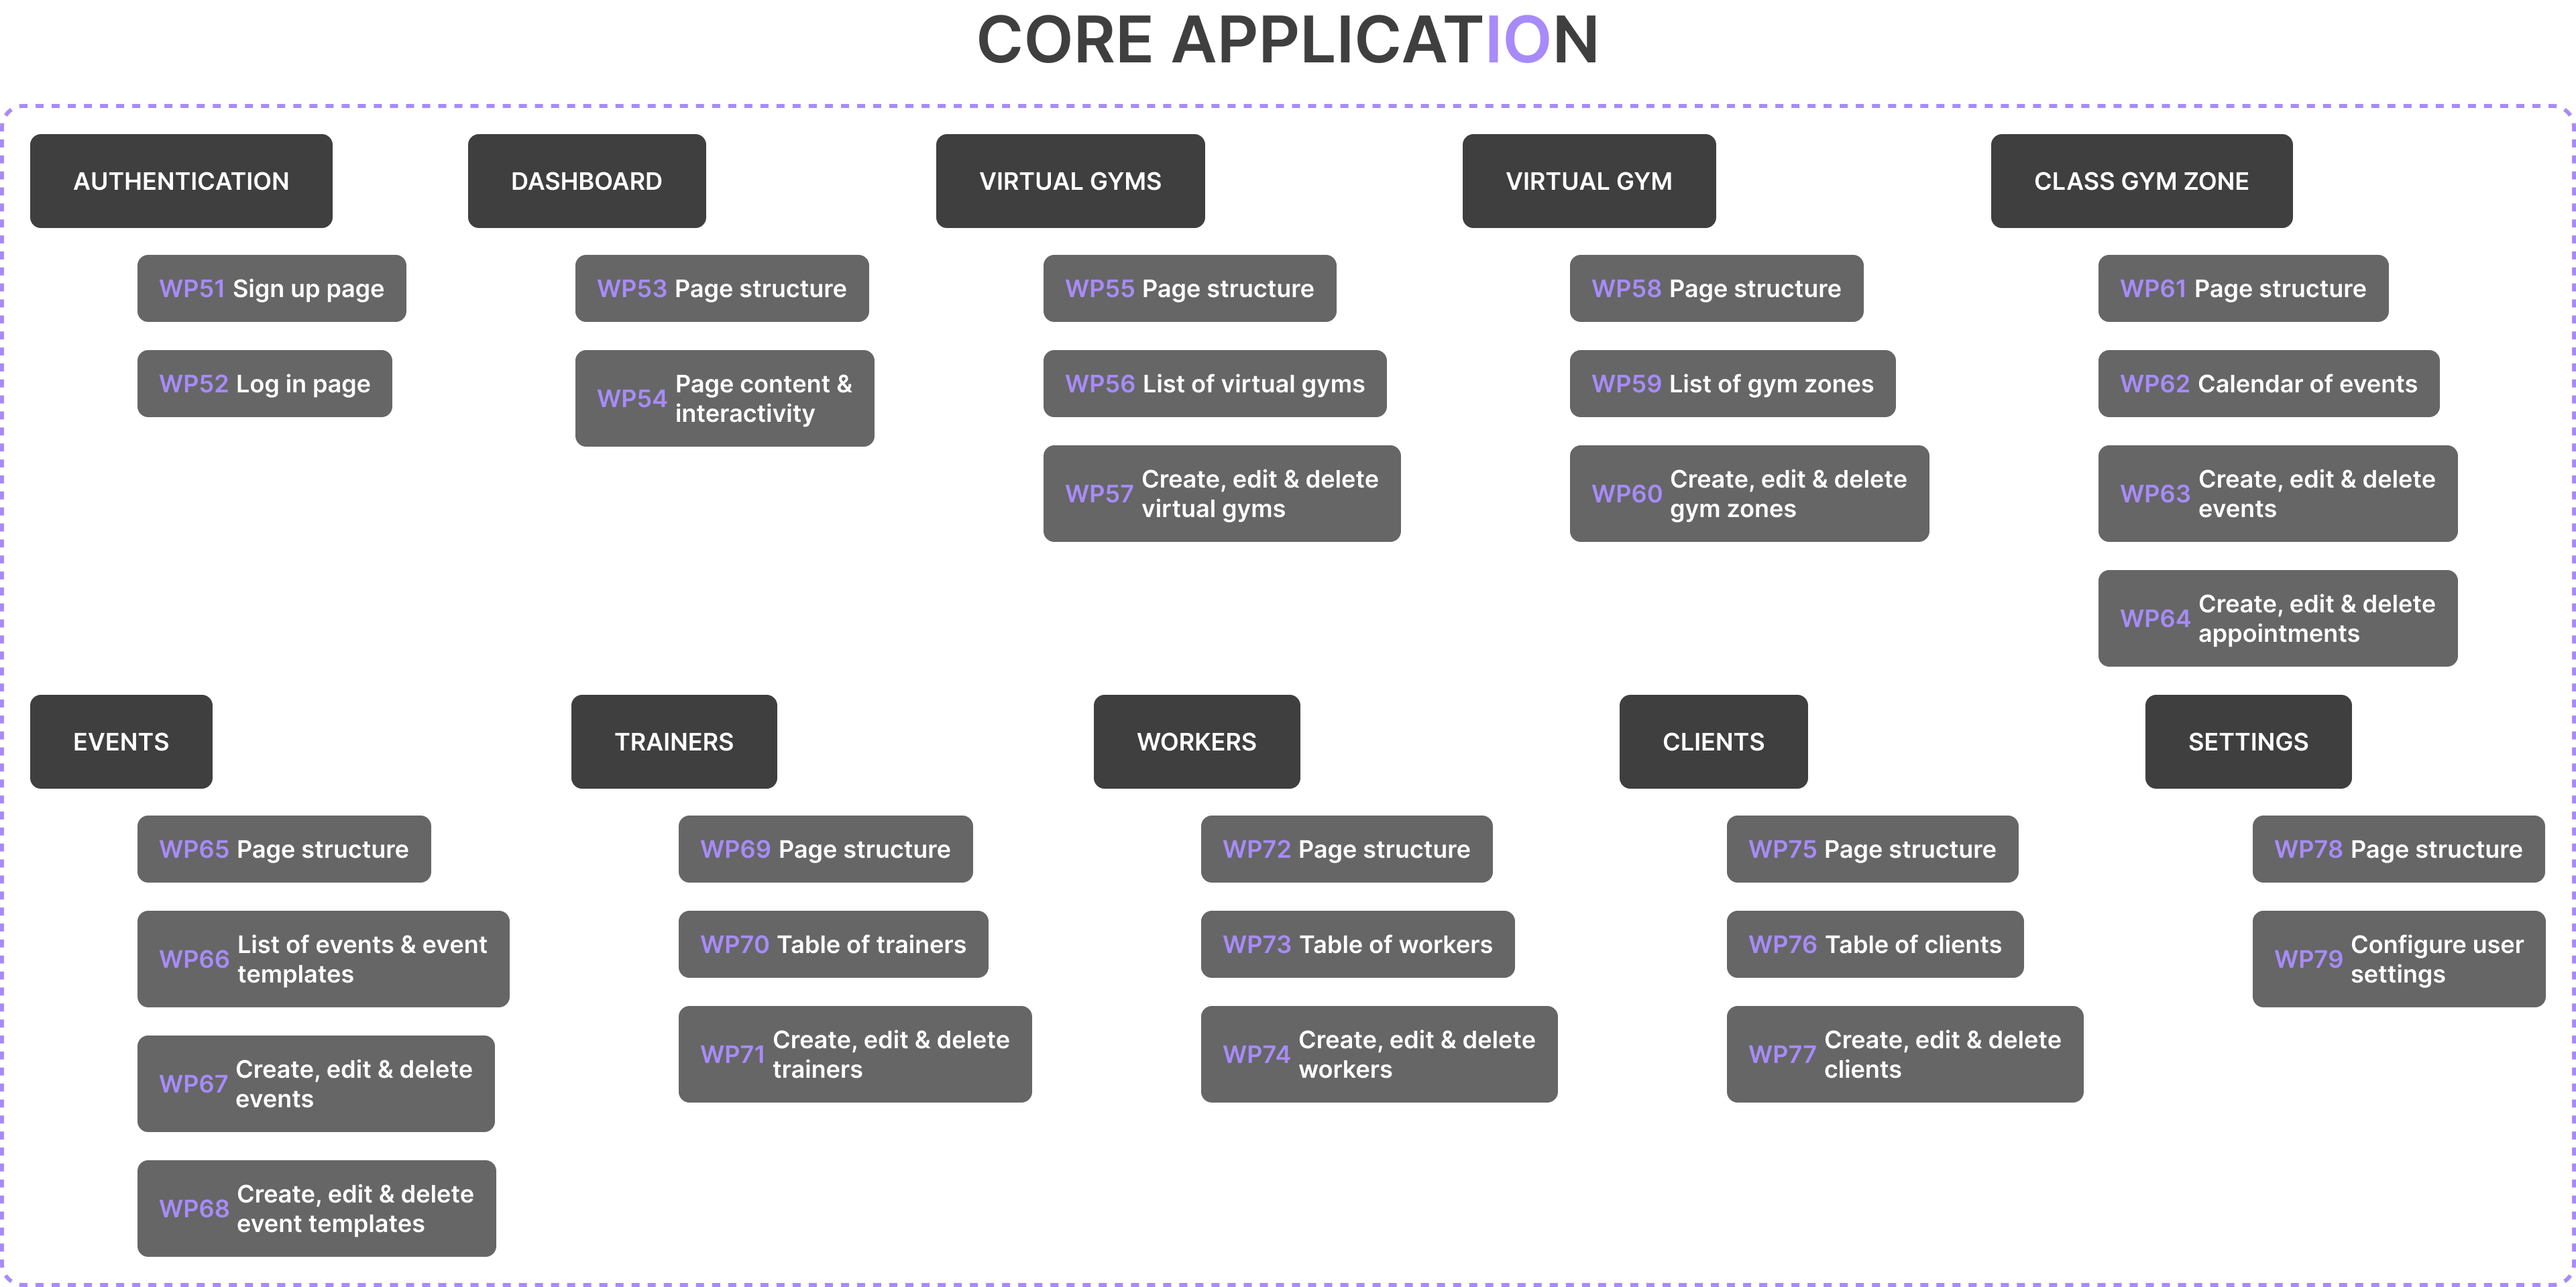
\includegraphics[width=\textwidth]{assets/working-packages/Core.png}
	\caption{Core application working packages diagram}
\end{figure}
\subsubsection{Client application}
\begin{figure}[H]
	\centering
	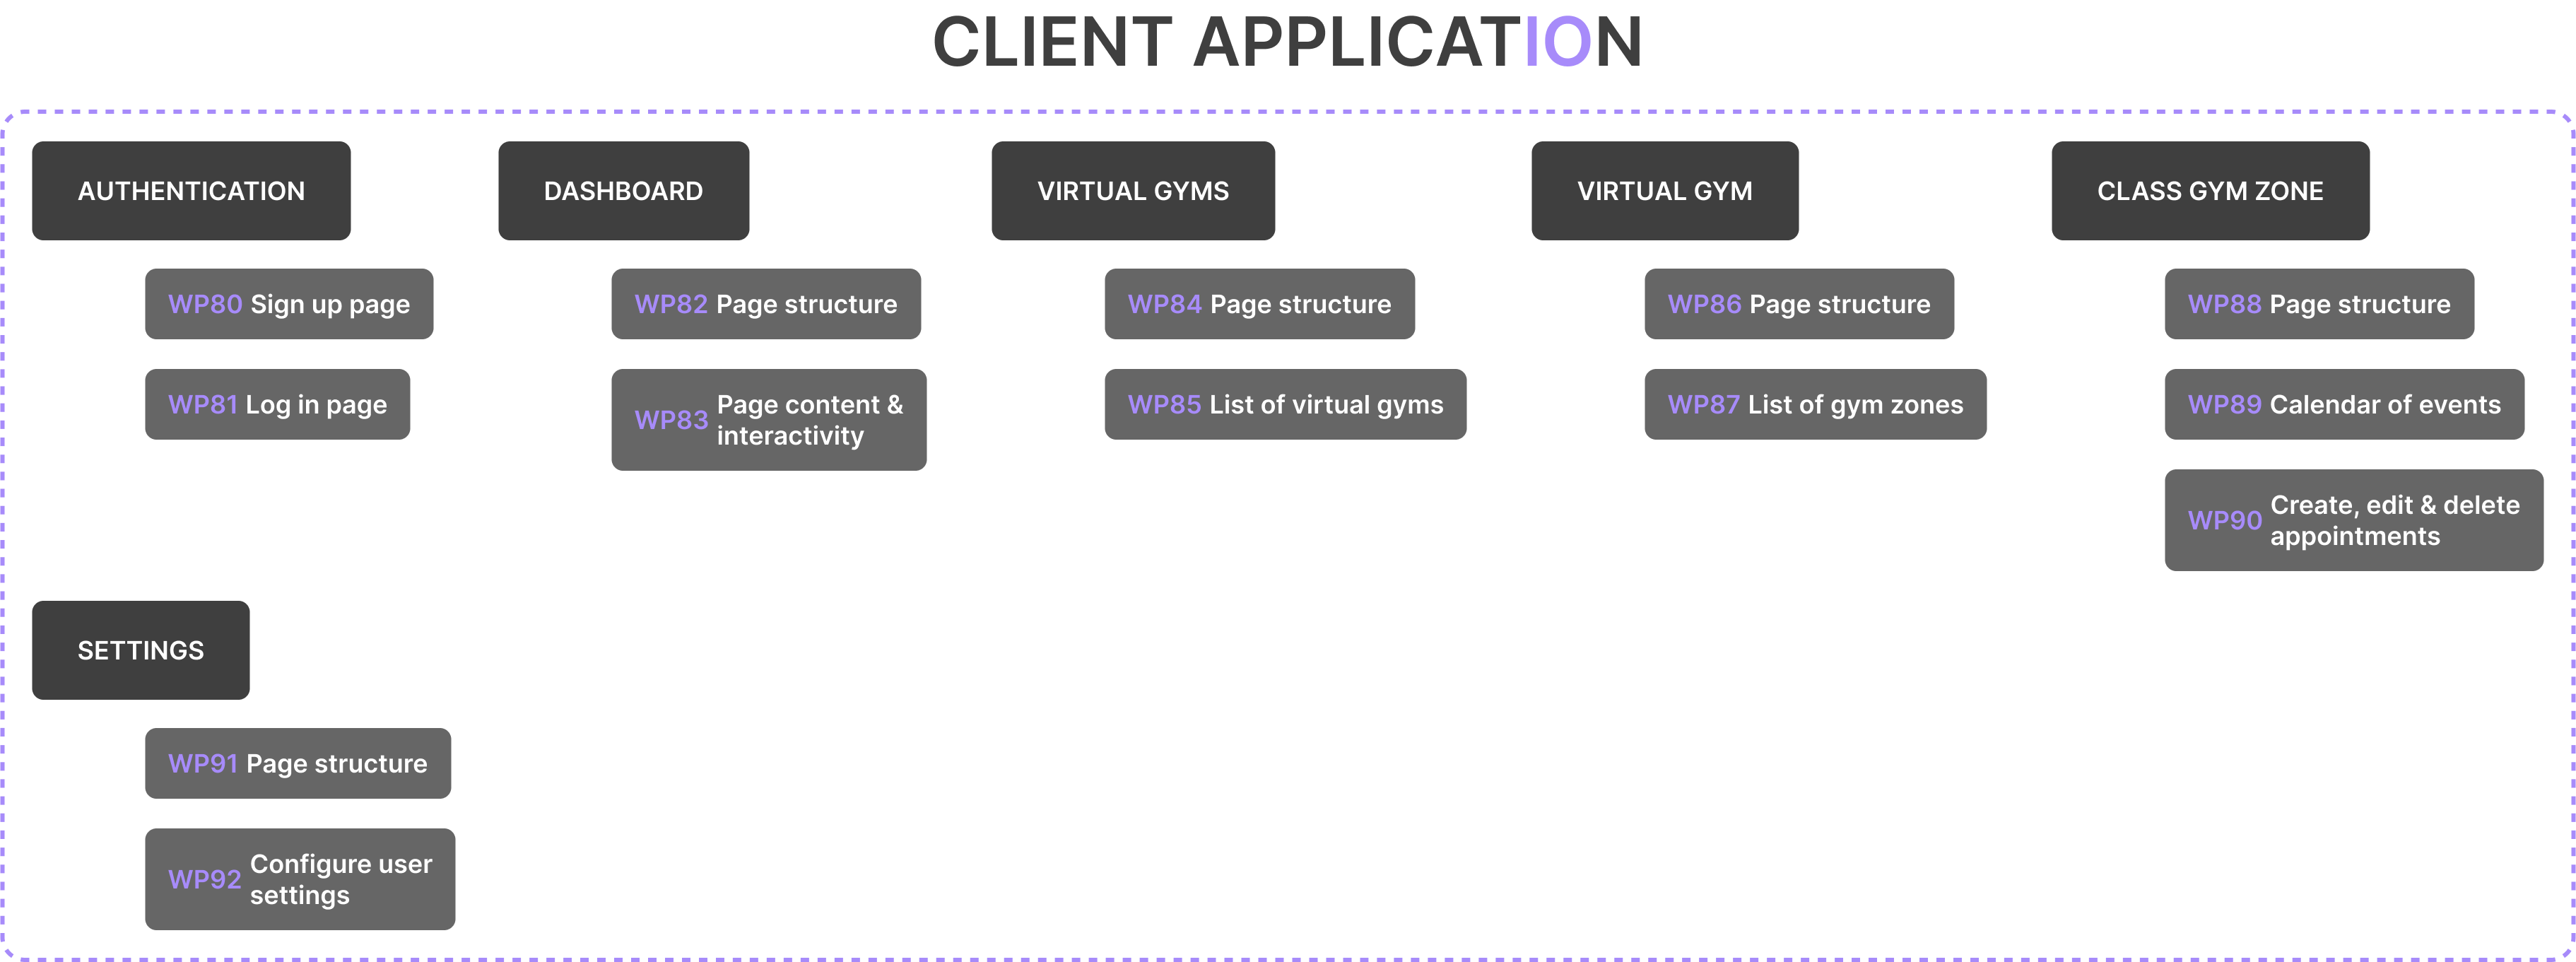
\includegraphics[width=\textwidth]{assets/working-packages/Client.png}
	\caption{Client application working packages diagram}
\end{figure}
\subsubsection{Landing application}
\end{document}